% !TEX root = ../../技术文档.tex
\section{NPU设计}

\subsection{NPU微架构}

NPU由计算图执行器、PE计算通路、算子控制器、片上缓冲、DMA、卷积窗口生成、辅助算子、定点后处理和整帧寄存器接口组成。
激活按算子记录选择UINT8或INT8，权重为对称INT8，完整卷积和与Bias采用INT32数据格式。
CPU通过MMIO提交整帧任务，绑定模型程序、工作区和本帧输入输出槽；NPU读取模型程序，解析算子及张量引用，依次完成各层计算和写回。
CPU在整网执行及检测后处理期间持有帧槽和模型工作区，在九个检测头发布后读取结果，完成框解码、NMS和主人脸选择。

整体结构如图\ref{fig:npu-microarchitecture}所示。DMA经AXI4连接外部存储，将输入特征图和权重搬入多存储体片上缓冲，并将输出特征图写回。
数据流控制模块（Data Streamer）按算子配置组织特征、权重、Bias及重定标参数输入，以及计算结果的输出通路，使供数顺序与计算单元所需的操作数顺序一致。
首层直接读取Video写入的模型输入槽，中间张量保存在共享DDR工作区，CPU只配置地址和任务身份。

\begin{figure}[!htbp]
\centering
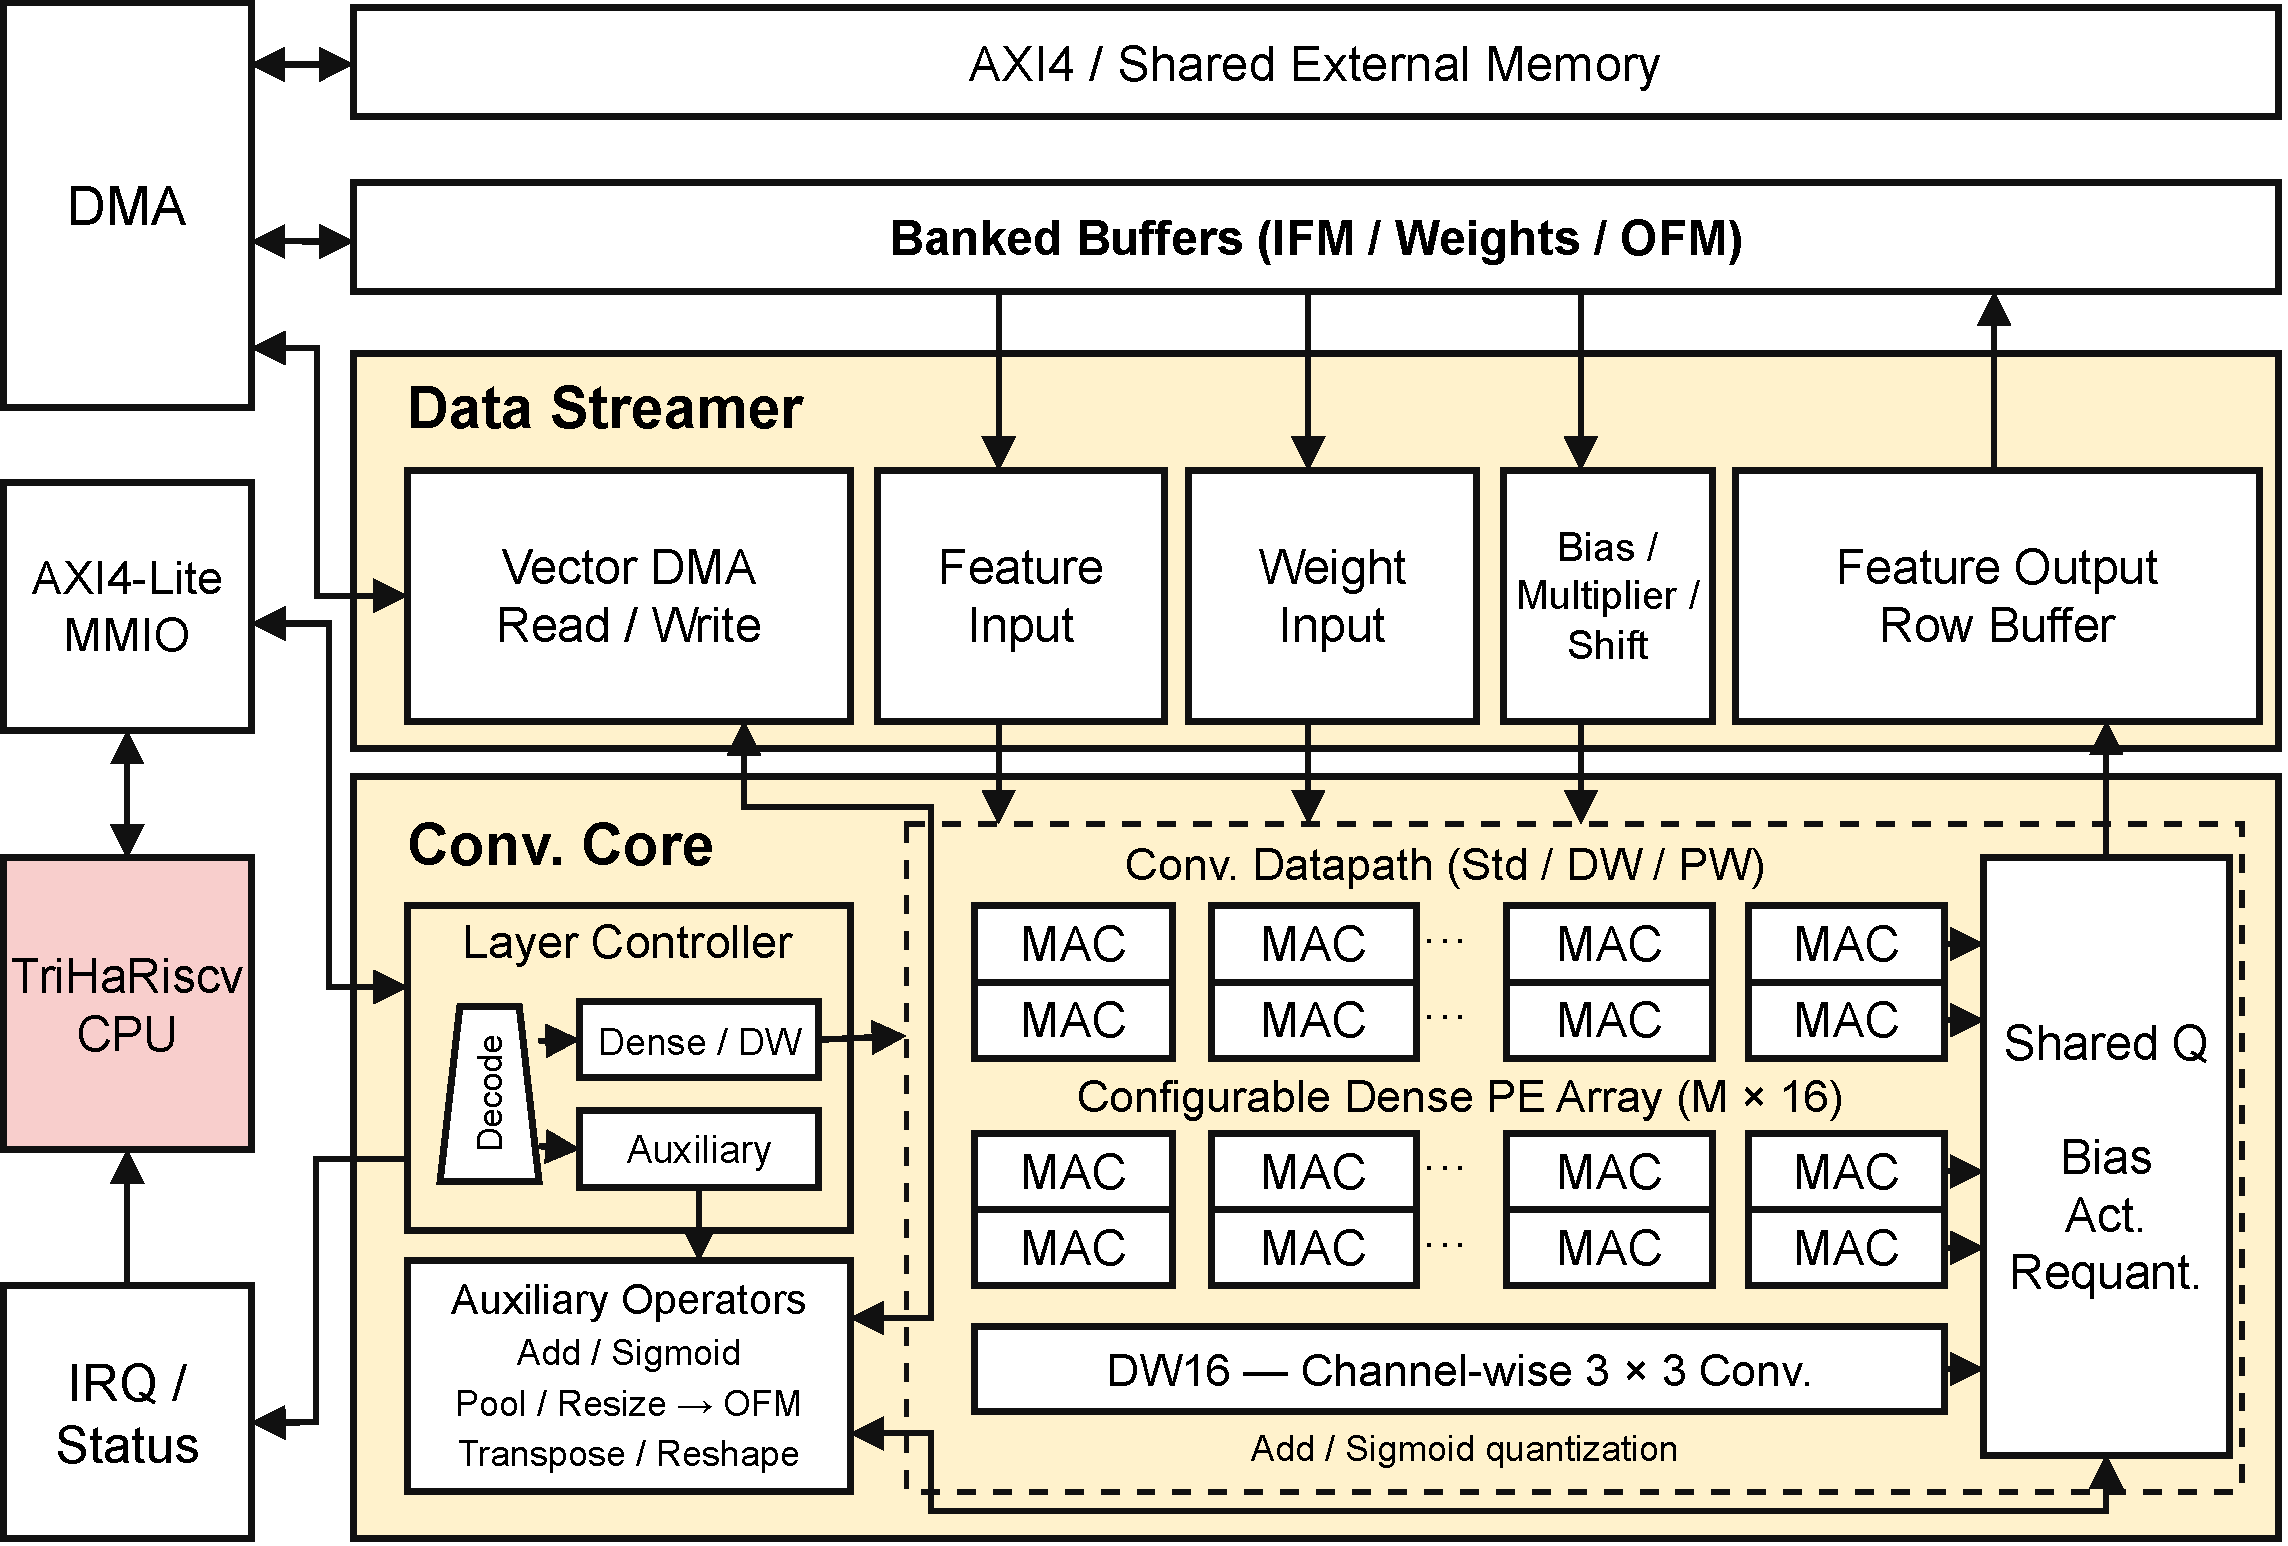
\includegraphics[width=\linewidth,height=0.78\textheight,keepaspectratio]{../figure/npu-microarchitecture.pdf}
\caption{NPU微架构}\label{fig:npu-microarchitecture}
\end{figure}

卷积核心采用可配置并行MAC阵列（Configurable PE Array）。普通卷积使用激活、权重广播和本地累加，
PE之间不逐级转发操作数或部分和，属于广播式并行结构。深度卷积使用独立的16通道乘加通路。
两条卷积通路共用定点后处理单元，累加结果经过Bias、重定标和饱和后送回输出缓冲。
Add与Sigmoid通过请求和返回接口使用同一量化通路；池化、缩放和张量重排按各自的数据路径完成读写。
图中的Host CSRs表示CPU经MMIO访问的NPU控制状态寄存器，数据流控制与卷积核心分别管理搬运和计算参数；整帧控制层组织计算图执行，并通过状态及中断接口报告任务结果。

单个算子的执行依次经历参数锁存、输入与权重搬入、窗口供数、计算、重定标和输出写回。
算子执行期间保持参数稳定，计算图执行器依据层完成状态推进下一算子。
整图执行结束、DMA无在途事务且外部服务适配器允许发布后，寄存器接口保持整帧完成记录。
CPU核对命令号、帧号、会话标识及发布状态，完成后处理后通过ACK释放记录；整帧执行期间共享工作区保持独占。

NPU路线采用硬件与模型协同设计，流程如图\ref{fig:npu-design-flow}所示。
设计输入包括FPGA计算与存储资源约束，以及YuNet ONNX模型的算子类型、张量形状和数据量分析，据此确定计算并行度、缓冲组织和算子映射。
硬件侧分别完成卷积核心与DMA、数据流控制、缓冲模块的RTL设计，集成后进行仿真、综合和布局布线。
模型侧准备校准数据，完成INT8校准、层与分块映射及模型量化，导出与硬件配置匹配的权重和参数。
两条流程在FPGA功能验证阶段汇合，结合检测精度与执行时延评价设计结果。

\begin{figure}[!htbp]
\centering
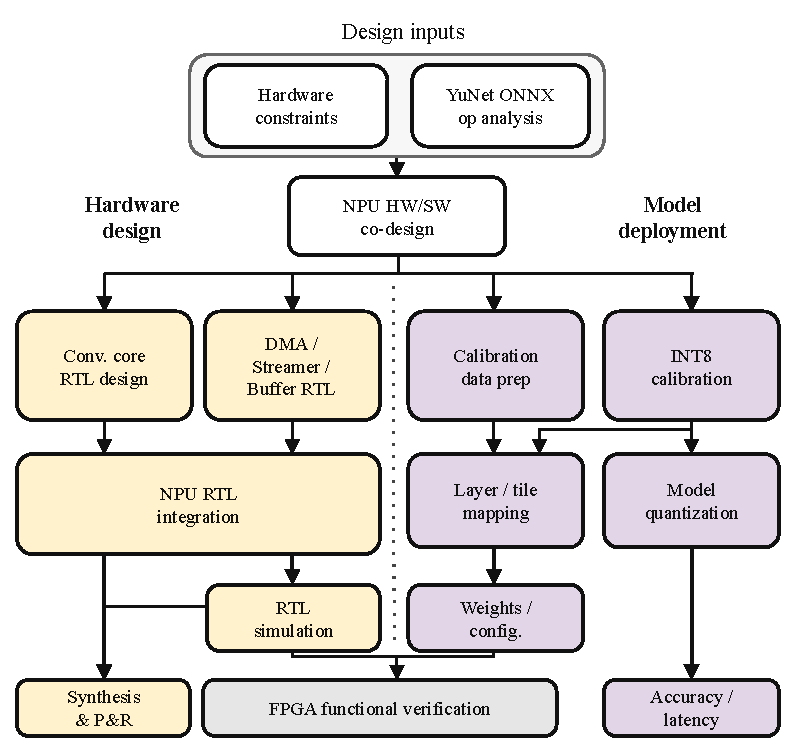
\includegraphics[width=\linewidth,height=0.78\textheight,keepaspectratio]{../figure/npu-design-flow.pdf}
\caption{硬件与模型协同设计流程}\label{fig:npu-design-flow}
\end{figure}

\subsection{PE计算单元}

乘法输入由激活类型决定：UINT8激活零扩展，INT8激活符号扩展，权重始终符号扩展。
首层直接执行U8$\times$S8，像素不减128；内部S8激活执行S8$\times$S8，融合ReLU后的U8激活仍执行U8$\times$S8。
阶段类型见表\ref{tab:npu-stage-types}。各阶段零点均为0，卷积补边使用数值0，不需要零点补偿项。

普通卷积阵列含$M$个空间位置、每位置16个输出通道，每个被接受的$K$向量完成$16M$次乘加。
每个APM的两条SIMD通路处理同一激活与相邻两个输出通道权重，阵列使用$8M$个APM。
板级配置取$M=2$，对应32次乘加/有效计算拍；模块默认$M=16$，对应256次乘加/有效计算拍。
空间并行度由综合参数\texttt{M\_LANES}设置，量化并行度由\texttt{QUANTIZER\_LANES}独立设置为1或2。
应用配置采用单量化通路，CPU与NPU共同运行于50\,MHz计算时钟。
运行时的形状、步长、有效掩码和地址来自算子记录。供数、后处理和写回开销由控制器另行承担。

每个累加器固定对应一个空间位置和输出通道，沿$K=C_{\rm in}K_hK_w$归约。
普通卷积限定$K\leq128$、权重范围为$[-127,127]$，原始和的绝对值不超过$128\times255\times127=4\,145\,280$，
因此APM内部使用24位有符号累加，结束后符号扩展到INT32接口，再加Bias。
深度卷积为16个通道各保留一个INT32累加器。有效掩码屏蔽尾通道和尾空间位置，输入有效与计算使能共同控制状态更新。

\subsection{卷积计算通路}

卷积计算通过片上保存与复用输入、权重和部分和，减少重复的外存访问\cite{sze2017efficient}。
普通卷积沿输入通道和卷积窗口完成归约，沿输出通道和输出空间位置分配并行工作。
1$\times$1卷积省去空间窗口展开，3$\times$3卷积由窗口收集器把当前空间块整理到激活缓冲A。
权重缓冲B按“输出通道块、$K$索引、16通道”排列，每个$K$索引同时读出一组激活和16个权重。
激活广播到16个输出通道，同一权重广播到$M$个空间位置；部分和始终保留在对应PE内。
完整$K$结束后才后处理，不在DDR中生成完整Im2Col矩阵，也不采用跨$K$块的部分和回装。

以首层普通3$\times$3卷积为例，输入为$3\times320\times320$，输出为$16\times160\times160$，步长2、四边各补1，$K=27$。
取板级$M=2$时，一个计算块覆盖同一输出行的两个相邻位置和全部16个输出通道。
DMA先把432\,B有效权重及Bias、重定标系数搬入片上缓冲；输入ROI保留各通道所需的三行，步长2换行时保留一行并补入两行。
窗口收集器按$(c,k_y,k_x)$顺序生成27个A向量，每向量含两个有效激活。
每个有效计算拍读取一个A向量和一个B向量，32个本地累加器分别归约27项，得到32个输出，计864次有效乘加。
边界越界位置的激活为0。权重保留供全层各空间块复用；当输出通道超过16时，同一A块还可供后续输出通道块复用。

以其后的首个深度3$\times$3卷积为例，输入、输出均为$16\times160\times160$，步长1、四边各补1，输入为S8。
每个空间位置对应一个16通道块，ROI的16个通道存储体同时提供同一窗口位置的16个激活，B提供16个对应权重。
8个SIMD APM完成每拍16次乘法，9个窗口位置依次进入各通道的INT32累加器，共144次有效乘加；此处不做跨通道归约。
通道块沿一整行扫描，九组权重反复读取；换到下一行时三行ROI轮换，只补入新的一行。
相邻窗口复用ROI中的像素，深度卷积直接读取ROI，不经过普通卷积的A展开。
DW16在首个核采样点以零为累加起点，中间采样点更新对应通道的部分和，最后一个合法采样点到达后提交结果。
通道掩码屏蔽尾部无效项，任务标签和有效位随计算流水传递，暂停期间保留尚未交付的结果。

上述两层均把量化后的结果写入O缓冲。16通道、160像素宽、U8输出时，O可容纳6个完整输出行，形成$16\times6\times160$的写回Tile，
最后一个Tile为4行。计算块的$M$个位置与写回Tile的行数分别由并行度和缓冲容量决定。
计算结果经量化写入O缓冲，当前写回Tile完成后才复用该缓冲，以上乘加数只描述有效算术工作量。

\subsection{算子控制器}

计算图执行器按模型记录生成层任务，算子控制器锁存形状、核尺寸、步长、补边、张量地址及量化参数，按算子类型选择普通卷积、深度卷积或辅助运算通路。
普通卷积按输出行、空间块、16输出通道块和完整$K$循环；深度卷积按输出行、16通道块、空间位置和窗口位置循环。
执行前检查形状、通道关系、数据类型、参数范围及存储边界；普通卷积的$K$超过128或输出行超过缓冲容量时拒绝任务。

控制状态与DMA握手衔接，背压时保持地址、数据和计数状态。
当前写回Tile的计算与量化全部结束后启动搬出，完成响应通过检查后才复用O缓冲；最后一个Tile完成后报告算子结束。
层核结束后仍需等待DMA与外部适配器完成事务，层状态交回计算图执行器。
跨层依赖、张量引用及下一算子的启动由计算图执行器管理，执行错误随整帧完成状态返回CPU。

\subsection{片上缓冲}

片上ROI按16个通道存储体组织，每个存储体为$1024\times32$\,bit，逻辑容量64\,KiB。
A、B、O分别包含4个存储体，每个存储体为$1024\times32$\,bit，各16\,KiB；输入行暂存为单存储体4\,KiB，Bias与重定标参数另存于小型参数存储。
这些数值是逻辑容量，物理存储块占用还受端口和映射方式影响。部分和驻留在计算通路的累加寄存器内。

ROI在整张特征图满足存储体容量时采用驻留方式，否则滚动保留卷积所需的输入行。
A按$K$索引存放空间向量，B按$K$索引提供16输出通道权重，O通过存储体轮换和双端口接收量化输出并恢复连续NCHW写回顺序。
DMA装载、窗口整理、计算和写回分阶段交接缓冲所有权，行复用减少重复读数。
输入行命中驻留缓冲时直接向窗口生成器供数；权重读取以请求标签对应返回数据，响应受阻时保持数据与标签稳定。
参数缓冲按输出通道保存32位Bias、32位重定标乘数和6位移位数，每次选出八个通道供定点后处理使用。
通道有效位记录已装载的参数，本组参数成功装载后置位\texttt{param\_valid}，权重读取据此启动。

设输出通道数为$C_o$、输出宽度为$W_o$、每元素字节数为$b$，O缓冲按下式检查单行容量：
\[
\left\lceil\frac{C_o}{4}\right\rceil
\left\lceil\frac{W_o b}{4}\right\rceil\leq1024
\]
输出行写入器按张量顺序组织数据，依据有效位置、通道和元素宽度生成字节使能，保护尾块相邻的无效区域。
输入FIFO清空时复位占用计数和载荷有效标志，重新装载完成后才对外提供有效数据，防止旧任务字节进入新任务。
行复用、窗口供数和输出尾块的组件验证见附录\ref{sec:npu-tiling-validation}。

\subsection{DMA控制器}

DMA内部采用256\,bit块服务，每块1至16个32\,B数据字，按AXI4的4\,KiB边界约束\cite{arm-axi-ihi0022e}及尾部字节拆分。
SoC适配器把一个数据字转换为先低后高的两个128\,bit AXI4拍，每个INCR突发最多16拍。
块服务串行持有一个读或写命令，适配器在当前突发完成后再发出下一子事务。
输入取数、输出行写回和向量访存共用这一块传输服务。Vector DMA为Add、Sigmoid、Transpose和Reshape提供元素块读写接口。
本地数据字与AXI数据拍的宽度不同，适配器按转换后的拍数重新划分突发，同时检查最终DDR地址的边界。

读返回按目标缓冲写入，写事务等待B通道成功响应。输出行写回还请求同端口读回，按字节掩码比对后返回块完成。
该读回用于检查搬运结果，算子完成时的数据可见性由DMA和外部服务适配器共同确认。
背压不能改变已提交的事务信息，错误响应与任务标识一并上报。卷积窗口在片上生成。
独立读写桥的功能仿真与完成握手验证见附录\ref{sec:npu-dma-validation}。

\subsection{卷积窗口生成}

窗口生成器根据输入尺寸、有效通道、步长和补边计算输入地址，从片上缓冲提取3$\times$3或1$\times$1操作数。
图像边界使用量化零值填充，通道对齐区由有效掩码屏蔽。
深度卷积供数保持通道对应关系，普通卷积供数按输入通道归约顺序排列。

首层输入在DDR中为B、G、R三个连续平面，每行320\,B、每平面102400\,B，总计307200\,B。
视频输入的上下各40行在NCHW写入时填0；卷积窗口超出$320\times320$张量时由供数逻辑另行补0。
两种补边均对应零点0，但发生在不同阶段。通道块尾部另以有效掩码屏蔽。
输入行读取模块按需装入行片，窗口生成器依据核位置、步长和补边选择本拍激活。
普通卷积将采样值组织为$M$个空间位置的向量；深度卷积按通道组提供同一核采样点的激活；池化和缩放按采样坐标取值。

\subsection{辅助算子单元}

辅助算子单元完成Add、Sigmoid、MaxPool、Resize、Transpose和Reshape，算子控制器按记录选择向量执行或空间采样。
Add通过向量端口读取两路输入，调用共享量化器完成尺度系数乘法，在宽中间域求和后统一舍入与限幅，再写回输出。
Sigmoid先将S8输入重定标为查表索引，读取模型包中的概率表，输出U16 Q0.16数据。CPU直接读取概率头用于后处理。
Add与Sigmoid的请求、返回均使用有效与接收握手；辅助系数读返回先保存于接收寄存器。
运算暂停期间保持已接收的系数，恢复后再更新供算子使用的参数。

MaxPool按2$\times$2窗口、步长2、无补边取最大值，输出尺寸向下取整。
Resize采用2倍最近邻上采样，按非对称坐标映射向下取整选择源位置。两者保持输入编码，采样结果进入O行缓冲，经行写入器提交DMA。
Transpose按部署记录支持的维序生成读写地址，Reshape保持元素顺序，按目标地址和长度搬运。
这两类操作通过向量端口读写原编码数据，不引入新的量化边界；支持的形状和维序由算子准入检查限定。
辅助算子的组件状态波形及数值比较结果见附录\ref{sec:npu-aux-validation}，各用例按其量化通路配置统计。

\subsection{定点后处理单元}

定点后处理接收INT32累加结果，完成Bias相加、整数系数乘法、移位、舍入与饱和。
融合ReLU的特征图输出为UINT8，非ReLU特征图输出为对称INT8，检测框回归输出为INT16；输出类型由算子参数选择。
权重采用逐输出通道尺度，激活采用逐张量尺度，相关系数随模型包装载。

BN在线下融合到权重与Bias，运行时使用融合后的整数参数。
完整$K$归约后只加一次Bias、重定标一次。重定标采用正INT31乘数、64位整数乘积及1至62位右移，按最近偶数舍入后依输出类型饱和。
UINT8范围为$[0,255]$，对称INT8为$[-127,127]$，INT16回归值为$[-32767,32767]$。
最近偶数舍入同样处理负半值，例如$-9/2=-4.5$舍入为$-4$，随后再执行目标类型的限幅。
量化接口每组包含八个元素，内部以一条或两条物理通路分时处理，并保留位置标签、有效掩码和输出类型。
Sigmoid概率采用U16 Q0.16编码，尺度为$2^{-16}$，数值1限幅至65535；其索引重定标与卷积共用量化硬件。
检测框解码与NMS由CPU执行，与本单元的张量重定标分开。
卷积累加、尾通道和定点后处理的组件验证见附录\ref{sec:npu-compute-validation}。

\subsection{寄存器接口}

整帧寄存器空间基址为\texttt{0x2000\,0000}，通过32位AXI4-Lite提供版本、能力、控制、状态、完成/错误中断及会话信息。
偏移\texttt{0x100}开始的32个32位字保存整帧任务，偏移\texttt{0x200}开始的20个32位字保存完成记录。
CPU写入程序、工作区、输入输出区域、几何参数及命令号、帧号和会话标识，执行I/O屏障后写START；接口在接收启动时原子锁存任务。
任务中的地址以共享窗口\texttt{0x8200\,0000}为基准提交字节偏移，计算图执行器据此绑定本帧数据。
内部存储服务使用相对DDR基址的地址，外部服务适配器加\texttt{0x8000\,0000}形成总线地址。

完成发布同时检查整帧执行结束、局部DMA空闲和外部服务适配器的发布许可。
接口进入\texttt{HELD}状态后保持完成记录，CPU核对执行状态、命令号、帧号、会话标识\texttt{epoch}及\texttt{published}标志。
应用配置的完成记录给出九头输出的地址与26,368\,B跨度，CPU在记录保持期间读取输出并执行检测后处理。
驱动通过轮询收取完成记录，硬件同时提供可使能的完成与错误中断。

CPU完成后处理并构建显示记录后，以匹配的命令号、帧号和会话标识ACK；确认NPU返回IDLE后，软件释放整图工作区并将帧置为待显示状态。
IRQ写1清除仅清除通知状态，活跃任务与待确认结果均锁定任务区；原图槽继续按显示引用管理。
任务执行错误、身份不符或会话变化使本次推理失效，软件保存错误并停止提交后续任务。
附录\ref{sec:npu-control-validation}给出单算子MMIO与输入FIFO的组件控制验证；整帧接口与应用循环的联合验证依据板级配置记录。

